\chapter{Wireframes}
\label{ch:wireframes}
When the app is launched it silently registers with the server
allowing the user to use the app immediately. The user is then shown
the middle-top screen.
\begin{enumerate}
\item From the middle top screen, the user can follow arrow 1 by
  clicking on the middle button "Pick Mission'' to pick a Mission
  (Run around Arran or Egg for example) and then pick a start and
  end location. After confirming these choices, the user is taken
  back to the middle top screen, or at any time can click the
  "Home'' button to return. 
\item The user can also view their current acheivements by clicking
  the "Achievements" button on the middle top screen, following
  arrow 2. These achievements will be grouped by tabs by category -
  Distance, Time, Stage and Mission based achievements.
\item The user can follow arrow 3 from the middle top screen to
  notify the app that they are starting an exercise period, telling
  the app to track their distance. If a Mission and start and end
  location are not picked (as in point 1) then they will instead be
  redirected to this screen and are unable to start exercising until
  this choice has been made. Once they have successfully advanced to
  this screen, it will display their current progress as they move
  showing the user how close to completion of their current stage
  and overall route they are. 
\item When the user has finished exercising, they will click the
  "End Session'' button and be taken to the first summary screen -
  following arrow 4. Here statistics from their exercise will be
  shown and the option to share this on several social media
  outlets.
\item The user can then move to the second and final summary screen,
  following arrow 5, where they will be shown any achievements they
  were awarded during that session. The user will also have the
  option to share these on social media outlets. From here, the user
  can click the "Home" button and be taken back to the middle top
  screen. 
\end{enumerate}
\begin{figure}[H]
  \centering
  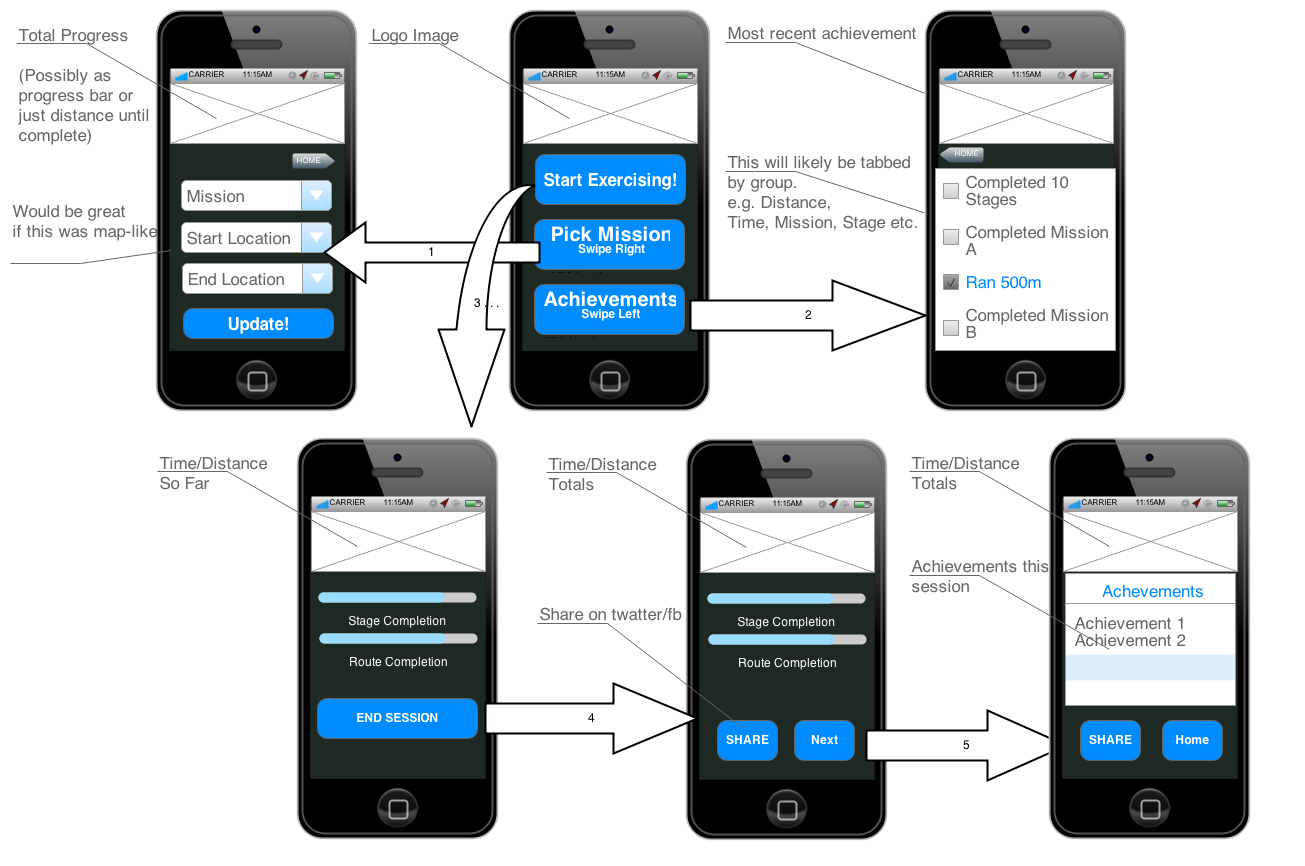
\includegraphics[width=\linewidth]{appendix/images/wireframes.png}
  \caption{Wireframes, initial design}
  \label{wireframes_1}
\end{figure}
\begin{figure}[H]
  \centering
  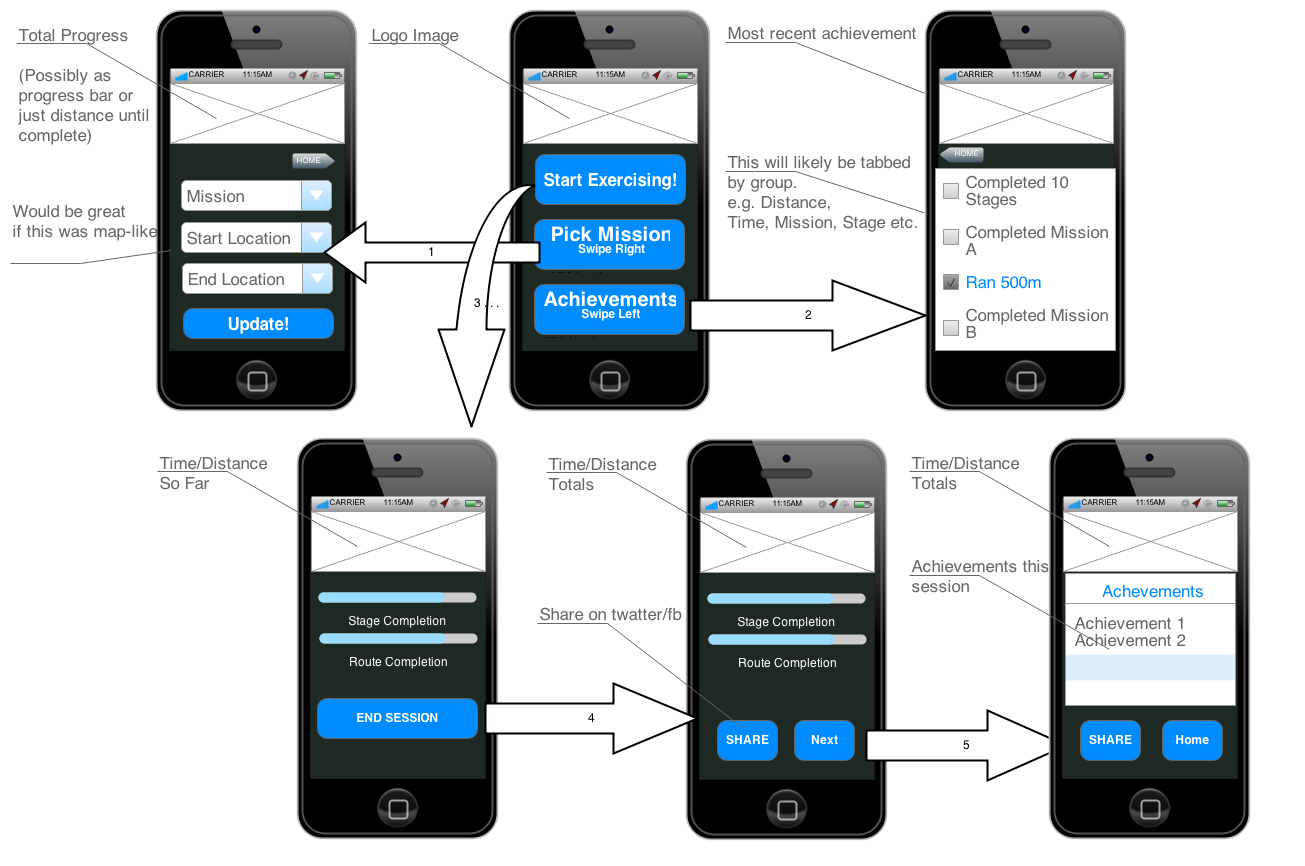
\includegraphics[width=\linewidth]{appendix/images/wireframes.png}
  \caption{Inital sketch of wireframe ideas}
  \label{wireframes_2}
\end{figure}

\chapter{Installation Instructions}

The code can be checked out using git by executing the following command in the terminal:

\noindent See the following command :
\begin{lstlisting}[language=bash]
  $ git clone git@github.com:marinamarina/sure-thing.git
\end{lstlisting}

Installation instructions are found at the following url:

\url{https://www.github.com:marinamarina/sure-thing/blob/master/README.md}.


If any issues arise regarding installation of any part of the
system, do not hesitate to contact me at 

1014481@rgu.ac.uk

\chapter{Project Specification}
Summary of the project outline.

\section{Functional Requirements}
some text here

\section{Non-Functional Requirements}
some text here

\chapter{Project Management}
Discussion on how the project was managed. What things impacted the success of the project. How does the continually revised versions of the project plan compare to the initial draft developed at the start of the project. Did everything run according the schedule. Did elements such as exams \& coursework have any impact. 


\chapter{Another Appendix}

This appendix makes use of the \emph{rotating} package to rotate both figures and tables ninety degrees allowing for large datasets and illustrations to be represented.

\begin{sidewaystable}
\begin{center}
   \begin{tabular}{llllllllll} 
   \toprule
   \textbf{Heading 1} & \textbf{Heading 2}  & \textbf{Heading 3}  & \textbf{Heading 4}  & \textbf{Heading 5}  & \textbf{Heading 6}  & \textbf{Heading 7}  & \textbf{Heading 8}  & \textbf{Heading 9}  & \textbf{Heading 10}  \cr
   \midrule
   aaa & bbbb & cccc & dddd & eeee & ffff & gggg & hhhh & iiii & jjjj \cr 
   aaa & bbbb & cccc & dddd & eeee & ffff & gggg & hhhh & iiii & jjjj \cr 
   aaa & bbbb & cccc & dddd & eeee & ffff & gggg & hhhh & iiii & jjjj \cr 
   aaa & bbbb & cccc & dddd & eeee & ffff & gggg & hhhh & iiii & jjjj \cr 
   aaa & bbbb & cccc & dddd & eeee & ffff & gggg & hhhh & iiii & jjjj \cr 
   aaa & bbbb & cccc & dddd & eeee & ffff & gggg & hhhh & iiii & jjjj \cr 
   \bottomrule
   \end{tabular}
\caption[A Short Caption for the table]{
	A much longer caption that will not be listed in the list of tables page.
}
\label{tab:sidewaysTable}
\end{center}
\end{sidewaystable}

\begin{sidewaysfigure}
\centerline{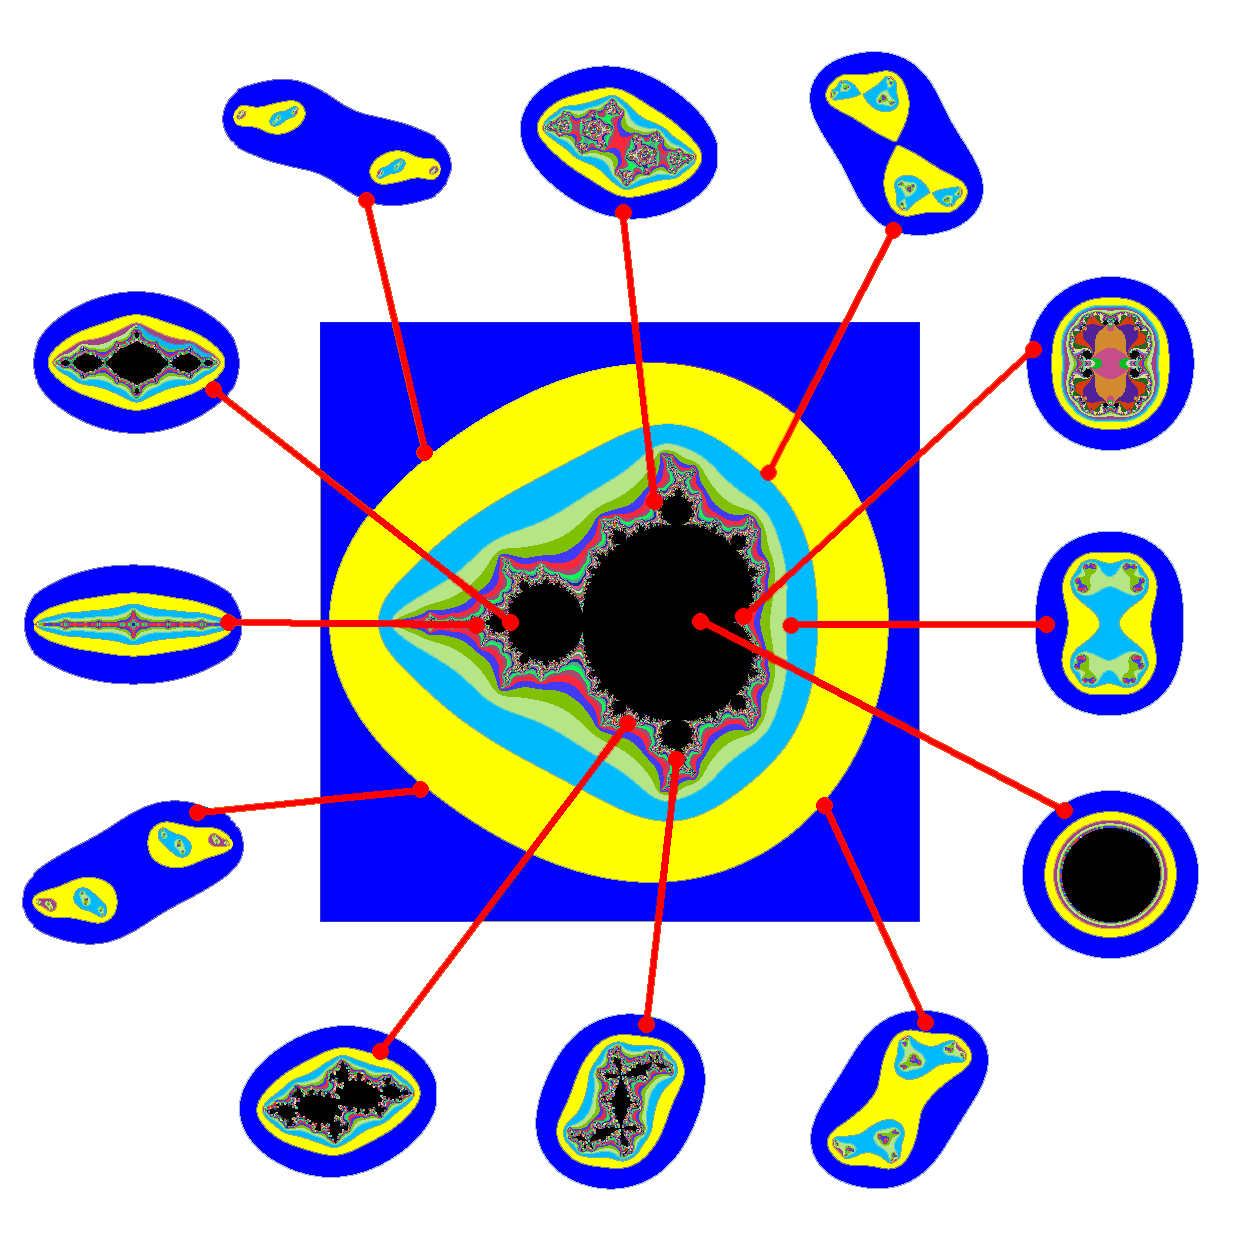
\includegraphics[width=0.8\textwidth,natwidth=610,natheight=642]{appendix/images/samplepng}}
\caption[A Sideways Figure]{
	A much longer caption that will not be listed in the list of figures page.
}
\label{fig:sidewaysFigure}
\end{sidewaysfigure}

\chapter{Implementation}

Third-Party Code and Libraries

The slides from the formal presentation should be provided here in not more than two pages. 

\chapter{Project Log}

The following is a weekly summary of the work carried during the development of this body of work. It covers tasks that were completed, tutorials that were worked through, articles that were read and reviews of discussions / meetings held with the project supervisor and other third parties. 

\section*{Week Beginning: Monday 27/09/2010}

First week working on the project. Had a meeting with supervisor and discussed some of the issues related to the project. The first deliverable is due for the end of next week (project outline \& ethics form). 

\begin{itemize}
  \item Downloaded and Installed \LaTeX \space (MikTeX full install), Ghostscript, Ghostview \& Winshell. 
  \item Started to get to grips with the \LaTeX \space system by making simple modifications to the template and editing the project log.
  \item Developed a Mind Map to clarify understanding of project elements.
  \item Prepared an initial draft of project plan in the form of a Gantt chart. 
  \item Prepared and revised 1 page draft of project summary \& filled in ethics form. 
\end{itemize}



